% ----------------------------------------------------------------
% AMS-LaTeX Paper ************************************************
% **** ---------------------------------------------------------
\documentclass[10pt,brazil]{exam}
\usepackage{geometry}
\geometry{verbose,tmargin=1.5cm,bmargin=1.2cm,lmargin=1cm,rmargin=1.5cm}
\usepackage[T1]{fontenc}
\usepackage[utf8]{inputenc}
%\usepackage{babel}
\usepackage{amsmath}
\usepackage{amsfonts}
\usepackage{mathtools}
\usepackage[usenames,dvipsnames]{pstricks}
\usepackage{amssymb}
\usepackage{amsthm}

%\usepackage[svgnames]{xcolor}
\usepackage{listings}

% Para redefinir o texto ao lado das pontuações:
\pointpoints{ponto}{pontos}


\usepackage{graphicx}

\usepackage{booktabs}

\usepackage{caption}

\usepackage{enumerate}

\setlength{\parindent}{0pt}

\usepackage{mleftright} % corrects spacing after \left( and before \right), etc
\mleftright

\newcommand{\E}{\mathbb{E}}
\newcommand{\Prob}{\mathbb{P}}
\newcommand{\T}{\mathbb{T}}
\newcommand{\prob}{\mathbb{P}}

\begin{document}
% Título do Artigo
\title{Gabarito Lista 4 }

% Definição do(s) autor(es). Observe que é possível colocar
% uma nota de agradecimento, ou algo semelhante.

\author{
  Prof. Marcio Valk \\
  Disciplina: Inferência B\\
  %\and
  %Author 4 and Author 5  \\
  %Institution B
 % \and
  %Author 5  \\
  %Institution C
  \date{}
}

% Data. Se você quiser, pode entrar com o texto desejado no campo \date
% Caso queira a data do dia da compilação, exclua o comando \date
% Caso não queira que nada seja impresso no lugar da data, use \date{}

\maketitle


\begin{enumerate}[1.]

\item %(Pg 33 e 34 apostila) -tem resposta
%Uma caixa contém 2 moedas. Uma apresenta cara com probabilidade 0,5 (equilibrada) e a outra apresenta cara com probabilidade 0,6 (viesada). Uma delas é escolhida aleatoriamente e lançada 3 vezes. Deseja-se saber se a moeda selecionada é a equilibrada ou a viesada.

\begin{enumerate}[a)]
\item Exemplo 2.3 da Apostila%Defina um teste para decidir entre $H_0:\theta=0.5$ e $H_1:\theta=0.6$.
\item Exemplo 2.5 da Apostila %Calcule as probabilidades de erro tipo I e II.
\end{enumerate}






\medskip
\item %(8.1 Casella and Berger) -tem resposta
% Em 1000 lançamentos de uma moeda, foram observadas 560 caras e 440 coroas. É razoável assumir que a moeda é equilibrada?
Se a moeda é equilibrada, $X\sim Binomial(1000,1/2)$.
 Use um teste de hipóteses para concluir que $p>1/2$.



\medskip
\item%(8.2 Casella and Berger) -tem resposta
 %Em uma determinada cidade o número de acidentes com automóveis em dado ano segue a distribuição de Poisson.
 %Nos últimos anos a média do número de acidentes por ano foi 15, e este ano foi 10. É correto afirmar que o número de acidentes está diminuindo?
$X\sim Poisson(15)$.
Calcule $P(X\leq 10|\lambda=15)$. Essa probabilidade é grande? 





\medskip
\item%(8.13 Casella and Berger) -tem resposta
% Seja $X_1,\ldots,X_n$  i.i.d. uniforme($\theta,\theta+1$). Para testar $H_0:\theta =0$ versus (vs.) $H_1:\theta > 0$, temos dois testes concorrentes:

 %$$\phi_1(X_1): \mbox{ Rejeita } H_0 \mbox{ se } X_1> 0.95,$$
 %$$\phi_2(X_1): \mbox{ Rejeita } H_0 \mbox{ se } X_1+X_2> C,$$

\begin{enumerate}[a)]
\item 
O tamanho de $\phi_1$ pode ser obtido diretamente por 

\[\alpha=P(X_1>0.95)=0.05.\]


Para calcular o tmanho de $\phi_2$ precisamos encontrar a distribuição de $Z=X_1+X_2$, sendo que $X_1\sim U(0,1)$ e $X_2\sim U(0,1)$. Observe na figura (histograma), que foi gerada com o código 
\begin{lstlisting}
# Gerando uniformes
x1=runif(100000,0,1)
x2=runif(100000,0,1)
z=x1+x2
hist(z,freq=F,breaks=60,main=expression("Z =" ~ X[1]+X[2] ~ ",  " ~ X[1] ~ "~U(0,1) " ~ ",  " ~ X[2] ~ "~U(0,1) "), ylab=expression(f[Z](z)))
\end{lstlisting}

que a distribuição de $Z$ em questão é uma distribuição triangular.

\begin{center}
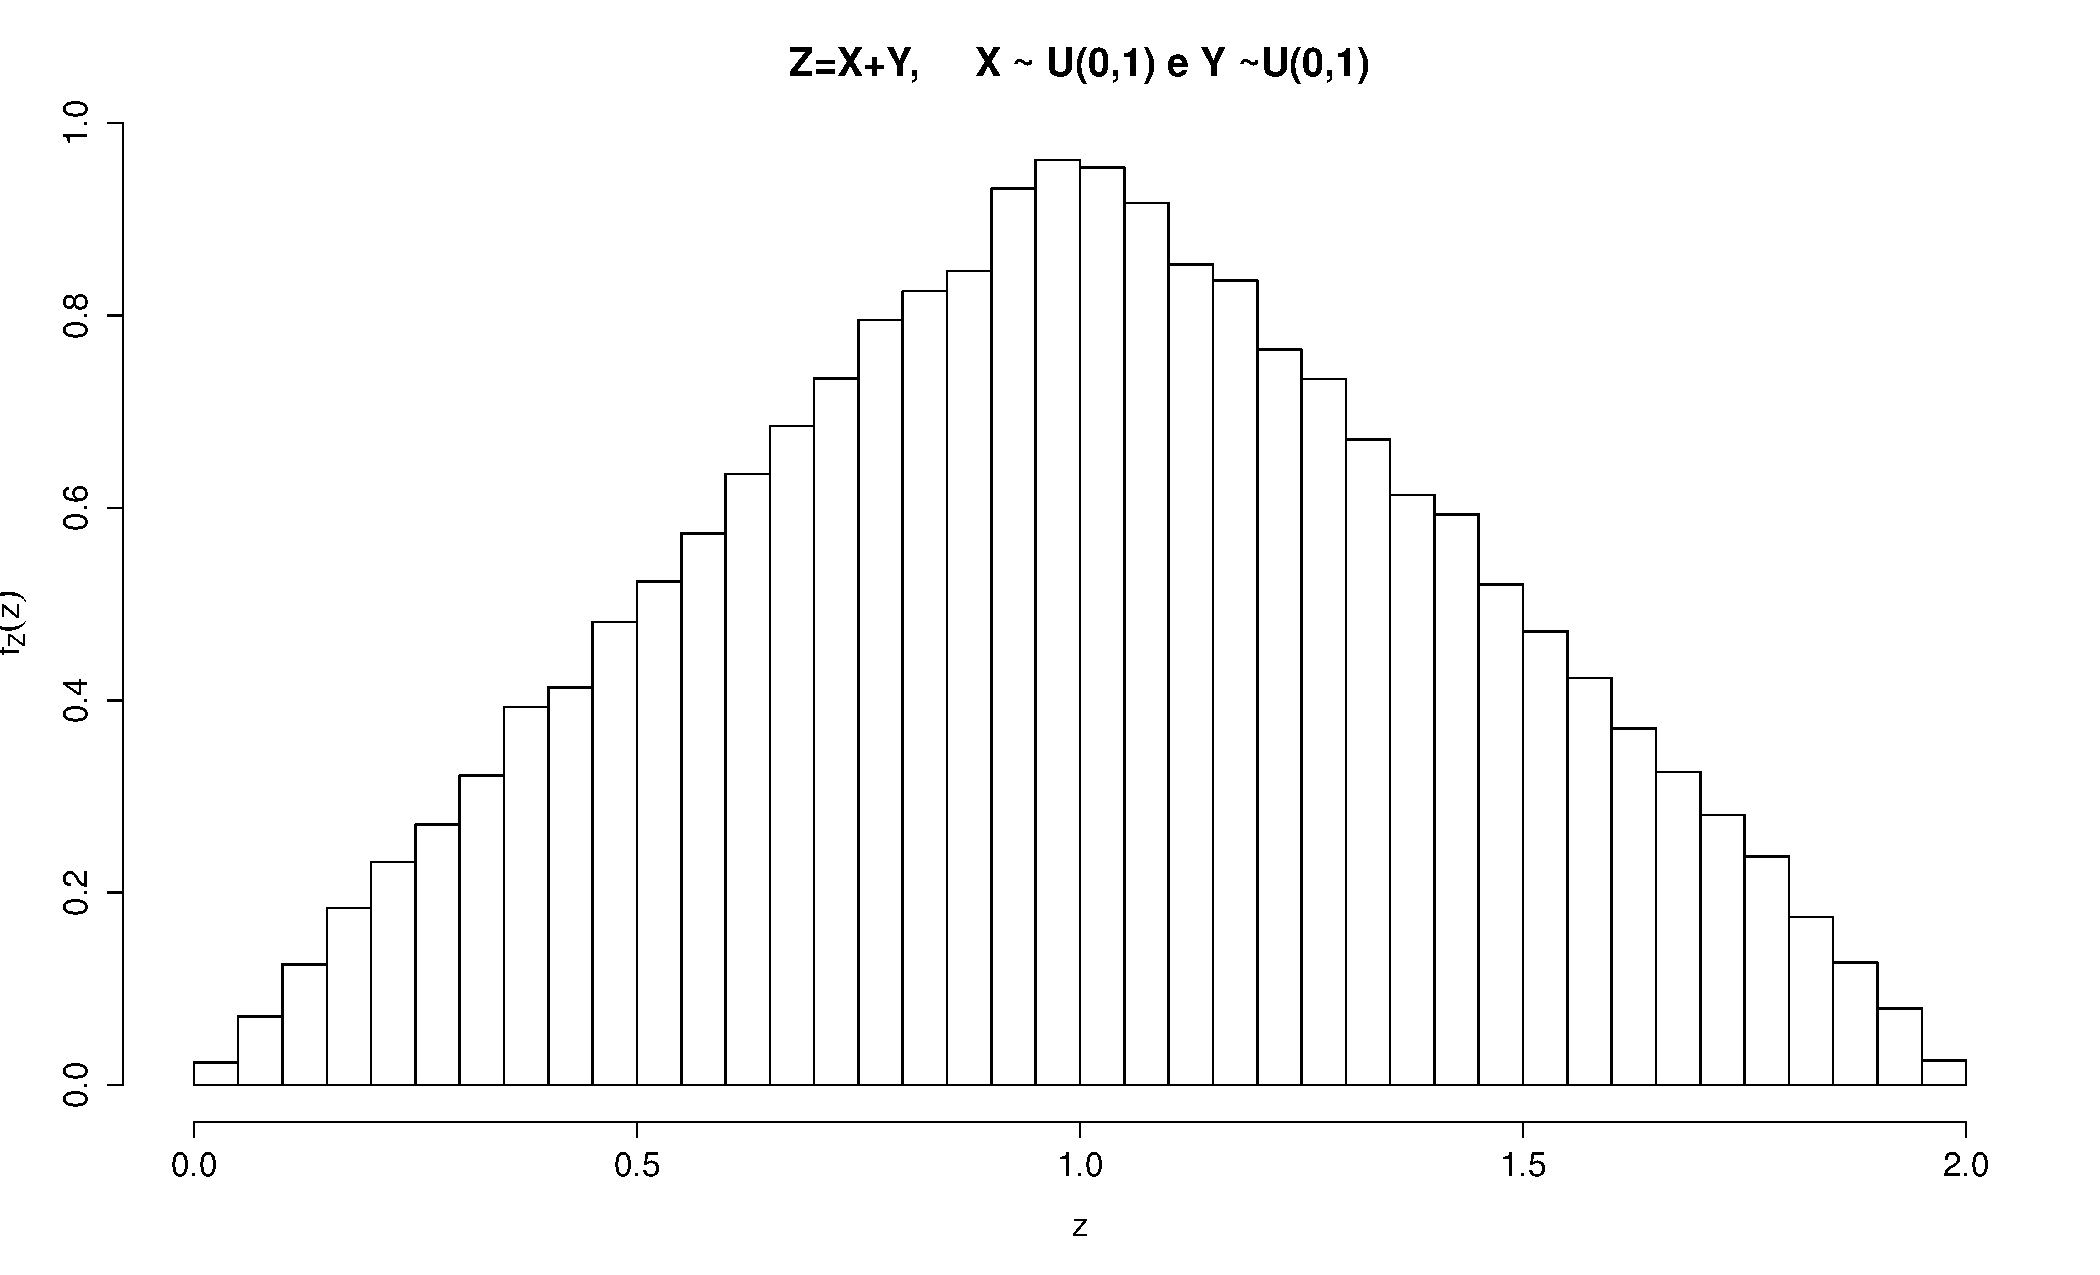
\includegraphics[scale=0.4]{sumunif.pdf} 
\end{center} 

Podemos usar a convolução para obter a densidade de $Z$. Assim, para $0\leq z\leq 2$

\begin{eqnarray*}
f_Z(z)&=&f_{X_1+X_2}(z)=
\int_{-\infty}^{\infty}f_x(x)f_Y(z-x)dx\\
&=&\int_{0}^{1}f_x(x)f_Y(z-x)dx
=\int_{0}^{1}f_Y(z-x)dx\\
&=&\begin{cases}
 \int_{0}^{z} f_Y(z-x)dx & \mbox{ se } 0\leq z< 1\\
 \int_{z-1}^{1} f_Y(z-x)dx & \mbox{ se } 1\leq z\leq 2\\
\end{cases}\\
&=&\begin{cases}
 z & \mbox{ se } 0\leq z< 1\\
 2-z & \mbox{ se } 1\leq z< 2\\
 0 & \mbox{ caso contrário.}
\end{cases}
\end{eqnarray*} 

Assim, para encontrar $C$ tal que $P(X_1+X_2 > C)=0.05$ é razoável/necessário assumir que $1\leq C\leq 2$. Logo

\[P(X_1+X_2>C]=P(Z>C)=\int_{C}^{1}(2-z)dz=\frac{(2-C)^2}{2}.\]




Segue que $\alpha=0.05$,  C= 1.68.%Encontre o valor de $C$ para o qual $\phi_2$ tenha o mesmo tamanho  que $\phi_1$.

\item    %Calcule a função poder de cada teste. Desenhe a função poder de cada teste.

\[\beta_1(\theta)=P_\theta(X_1>0.95)=\begin{cases}
 0 & \mbox{ se } \theta\leq -0.05\\
 \theta+0.05 & \mbox{ se } -0.05< \theta\leq 0.95\\
 1 & \mbox{ se } 0.95<\theta.
\end{cases}\]

Para encontrar a função poder do teste $\phi_2$ precisamos calcular a distribuição/densidade de $Z=X_1+X_2$ em que $X_i\sim U(\theta,\theta+1)$. Usando o fato que a densidade da soma $X_1+X_2$ é uma triangular entre $2\theta$ e $2\theta+2$, podemos escrevê-la como

\begin{eqnarray*}
f_Z(z)
&=&\begin{cases}
 z-2\theta & \mbox{ se } 2\theta \leq z< 2\theta+1\\
 2\theta +2-z & \mbox{ se } 2\theta+1\leq z <2\theta+ 2\\
 0 & \mbox{ caso contrário.}
\end{cases}
\end{eqnarray*} 


 
\[\beta_2(\theta)=P_\theta(X_1+X_2>C)
=\begin{cases}
0 & \mbox{ se } \theta \leq C/2-1\\
 (2\theta +2-C)^2/2 & \mbox{ se } C/2-1 < \theta \leq (C-1)/2\\
 1-(C-2\theta)^2/2 & \mbox{ se } (C-1)/2< \theta \leq C/2\\
 0 & \mbox{ se } C/2<\theta.
\end{cases}\]

Assuma que C=1.68 e faça os gráficos.

%=\begin{cases}
% 0 & \mbox{ se } \theta\leq -0.05\\
% \theta+0.05 & \mbox{ se } -0.05< \theta\leq 0.95\\
% 1 & \mbox{ se } 0.95<\theta.
%\end{cases}\]

\item  Observe nos gráfico que em algumas regiões o $\phi_2$   tem mais poder que o $\phi_1$ e em outras regiões o contrário acontece.
%$\phi_2$ é mais poderoso que $\phi_1$?

\item %Mostre como encontrar um teste que tenha o mesmo tamanho de $\phi_2$, mas que seja mais poderoso que $\phi_2$.

Uma opção é rejeitar $H_0:\theta=0$ também quando $X_1>1$ ou $X_2> 1$. Nesse caso o tamanho continua o mesmo do $\phi_2$ mas você rejeita em mais situações. Então seria mais poderoso que $\phi_2$.

\end{enumerate}


\medskip
\item  Resolvemos em aula
%(ex 3 mae3-l6 listas da net) -tem resposta
% Seja $X_1,\ldots,X_n$  a.a. de uma v.a. $X$ com função de densidade dada por
%
%\[f(x)=\theta x^{\theta-1},\,\,\,\,0<x<1,\,\,\,\theta> 0.\]
%
%\begin{enumerate}[a)]
%\item  Mostre que o teste mais poderoso para testar  $H_0:\theta =1$ vs. $H_1:\theta = 2$ rejeita $H_0$, se e somente se, $\sum_{i=1}^n -\log x_i\leq a$, em que $a$ é uma constante.
%
%\item Sendo $n=2$ e $\alpha=(1-\log 2)/2$, qual é a região crítica?
%\end{enumerate}



\medskip
\item %(ex 3 mae3-l6 listas da net) -tem resposta
% Seja $X_1,\ldots,X_n$ a.a. de uma v.a. $X$ com função de densidade $N(0,\sigma^2)$.
%
\begin{enumerate}[a)] 
\item %Encontre o teste uniformemente mais poderoso (UMP) para testar $H_0:\sigma^2 =\sigma_0^2 $ vs. $H_1:\sigma^2 > \sigma_0^2 $
O teste mais poderoso para esse teste alternativo será o de região crítica dada por

\[A^*=\left\{{\bf x};\frac{L_1({\bf x})}{L_0({\bf x})}\geq k\right\}\].

\[\frac{L_1}{L_0}\geq k \Leftrightarrow  \sum x_i^2\geq \log\left[k(\sigma_1^2/\sigma_0^2)^{n/2}\right]\left(\frac{1}{2\sigma_0^2}-\frac{1}{2\sigma_1^2}\right)^{-1}=c \]

Assim, o teste MP acima terá região crítica dada por 

\[A^*=\left\{\sum x_i ^2 \geq c\right\}\].

Como o teste acima vale para qualquer valor de $\sigma_1^2$ , ele  também será o teste UMP. 



\item %Seja $\alpha = 0.05$, $n = 9$ e $\sigma_0^2=9$.
 %Faça o gráfico da função poder.
 
 Observe que \[\sum \left(\frac{X_i}{3}\right)^2\sim\chi^2_{(9)}\]
 
 e 
 
 \[\alpha = P_{H_0}\left(\sum X_i^2 \geq c\right)=P_{H_0}\left( \sum\left(\frac{X_i}{3}\right)^2\geq \frac{c}{9}\right)\]
 
 Dessa forma, basta encontrarmos $c/9$ com o comando  $qchisq(0.95,9).$

 \[\frac{c}{9}=16.91898 \rightarrow c=152.2708.\]
 
 Segue que  a função poder é dada por \[\beta(\sigma^2)=P\left(X\geq \frac{152.2708}{\sigma^2}\right)\]
 em que $X\sim\chi^2_{(9)}$.
\end{enumerate}




\medskip
\item 
%%(8.12 Casella and Berger) -tem resposta
%Para amostras de tamanho $n=1,4,16,64,100$ de uma população normal com média $\mu$ e variância conhecida $\sigma^2$, faça o gráfico da função poder dos seguintes testes da razão de verossimilhança (TRV's). Tome $\alpha=0.05$.
\begin{enumerate}[a)]
\item %$H_0:\mu\leq 0$  vs. $H_1:\mu>0$.


Fazendo a razão de verossimilhanças encontramos que rejeita-se $H_0$ se $\overline{x}>\frac{c\sigma}{\sqrt{n}}$. Para $\alpha=0.05$ temos que $c=1.645$.

\[\beta(\mu)=P\left(\frac{\overline{X}-\mu}{\sigma/\sqrt{n}}>1.645-\frac{\mu}{\sigma/\sqrt{n}}\right)=P\left(Z>1.645-\frac{\sqrt{n}\mu}{\sigma}\right)\]

\item %$H_0:\mu= 0$  vs. $H_1:\neq 0$
Nesse caso rejeita-se $H_0$ se $|\overline{x}|>\frac{c\sigma}{\sqrt{n}}$. Para $\alpha=0.05$ temos que $c=1.96$.

\[\beta(\mu)=P\left(-1.96-\frac{\sqrt{n}\mu}{\sigma}\leq Z\leq 1.96+\frac{\sqrt{n}\mu}{\sigma}\right)\]

Use o R para fazer os gráficos. 
\end{enumerate}








\medskip
\item %(8.5 Casella and Berger) -tem resposta
 Uma a.a. $X_1,\ldots,X_n$ é retirada de uma população Pareto com densidade

$$f(x|\theta,\nu)=\frac{\theta\nu^\theta}{x^{\theta+1}}I_{\nu,\infty}(x),\,\,\,\theta>0,\,\,\,\nu>0.$$

\begin{enumerate}[a)]
\item %Encontre os EMV's de $\theta$ e $\nu$.
$\hat{\nu}=x_{(1)}$ e \[\hat{\theta}=\frac{n}{\log\left(\prod x_i/x_{(1)}^n\right)}=\frac{n}{T}\]
\item % Mostre que o TRV
%$$H_0: \theta=1,\,\,\nu\,\,\mbox{desconhecido},\,\,\,\,\,\,\,vs\,\,\,\,\,\,\, H_1: \theta\neq 1,\,\,\nu\,\,\mbox{desconhecido},$$
%tem região critica da forma $\{x:T(x)\leq c_1\,\,ou\,\,T(x)\geq c_2\}$, em que $0<c_1<c_2$ e $$T=\log \left[ \frac{\prod_{i=1}^{n}X_i}{(\min_i X_i)^n}\right].$$
\[\lambda({\bf x})=\frac{L_1({\bf x})}{L_0({\bf x})}=\left(\frac{T}{n}\right)^n e^{-T+n}.\]

Observe que $\frac{\partial}{\partial T}\log \lambda({\bf x})=(T/n) -1. $ Assim,  $\lambda({\bf x})$ é crescente para $T\leq n$ e decrescente para $T\geq n$. Ou seja, existe um $c_1$ e um $c_2$ tal que  $\lambda({\bf x})$ é grande se $T\geq c_1$ ou $T\leq c_2$.


\end{enumerate}





\medskip
\item Não Fazer

%
% %(8.6 Casella and Berger) -tem resposta
%Suponhamos que temos duas amostras de variáveis aleatórias independentes: $X_1\ldots,X_n$ são exp($\theta$) e $Y_1\ldots,Y_n$ são exp($\mu$). Encontre o TRV de $H_0:\theta=\mu$ vs. $H_1:\theta\neq \mu$.
%
%%\begin{enumerate}[a)]
%%\item Encontre o TRV de $H_0:\theta=\mu$ vs. $H_1:\theta\neq \mu$.
%%\item Mostre que o teste da parte a) pode ser baseado na estatística
%%$$T=\frac{\sum X_i}{\sum X_i+\sum Y_i}.$$
%%\item Encontre a distribuição de $T$ quando $H_0$ é verdadeira.
%%
%%\end{enumerate}









\medskip
\item  Não fazer %(8.8 Casella and Berger) -tem resposta
%Um caso especial da família de distribuições \emph{normal} é quando a média e a variância são relacionadas, como por exemplo a família $N(\theta,a\theta)$. Se estamos interessados em testar esse relacionamento, independente do valor de $\theta$, nos deparamos com um problema chamado problema do parâmetro ``nuisance''.
%
%\begin{enumerate}[a)]
%\item Encontre o TRV de $H_0:a=1$ vs. $H_1:a\neq 1$ baseado em uma amostra $X_1,\ldots,X_n$ de uma família $N(\theta,a\theta)$, em que $\theta$ é desconhecido.
%
%\item  Um problema similar ocorre quando a família é $N(\theta,a\theta^2)$. Assim, se  $X_1,\ldots,X_n$ são i.i.d. $N(\theta,a\theta^2)$, quando $\theta$ é desconhecido, encontre o TRV de $H_0:a=1$ vs. $H_1:a\neq 1$.
%\end{enumerate}
%





\end{enumerate}

\end{document}
% ----------------------------------------------------------------
